 \chapter{Energy Model}
 
 The first step in making an energy model of the GPS is to analyze the data from the measurements and relating it to the theory. The theory section explains how the receiver operates between two distinct phases: acquisition and tracking. The two phases can be modelled in a state diagram. 
 
 
 \begin{figure}[H]
\centering
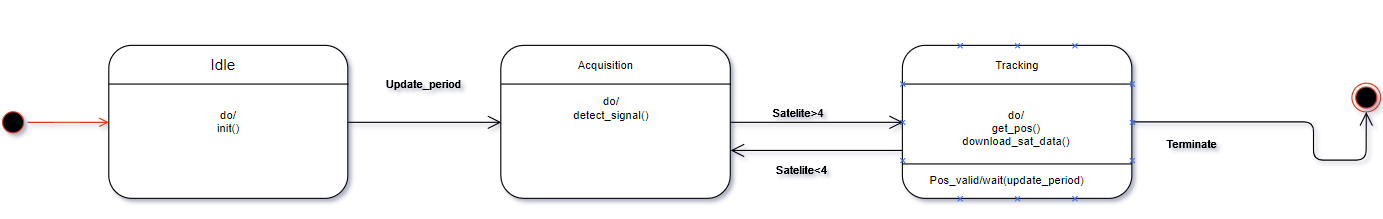
\includegraphics[width=16 cm]{Project_Report/Images/gps_basics.PNG}
\caption{The state diagram of a GPS receiver}
\label{fig:GPS reciever}
\end{figure}
 
 The trigger functionality from ref highlights when the receiver has a positional fix and when it is in the initial tracking state. It can't however inform about later transitions, because the GPS changes phases after it has a positional fix. The receiver does this to maintain its signal strength. The data from \cite{L76} is therefore compared to the ref waveform to validate the state diagram. 
 
 
 
 The waveform ref shows how the initial current consumption after fix. The voltage decreases which is the excepted behavior when the reciever . It also shows how the receivers 
 
 But by using the data from \cite{L76} and comparing it to the current consumption
 
 
 By using the current consumption of the GPS and comparing it with the data from \cite{L76}.
 
 
 which state the GPS receiver is in after the initial trigger because the trigger is based on the , since the trigger is based on the status of fix. 
 
 
 
 It is known that the GPS transitions between two states: Acqusition and Tracking. We used this states to build a 
 
 
 
 
 The state diagram of the LoPy is shown in figure:
\begin{figure}[H]
\centering
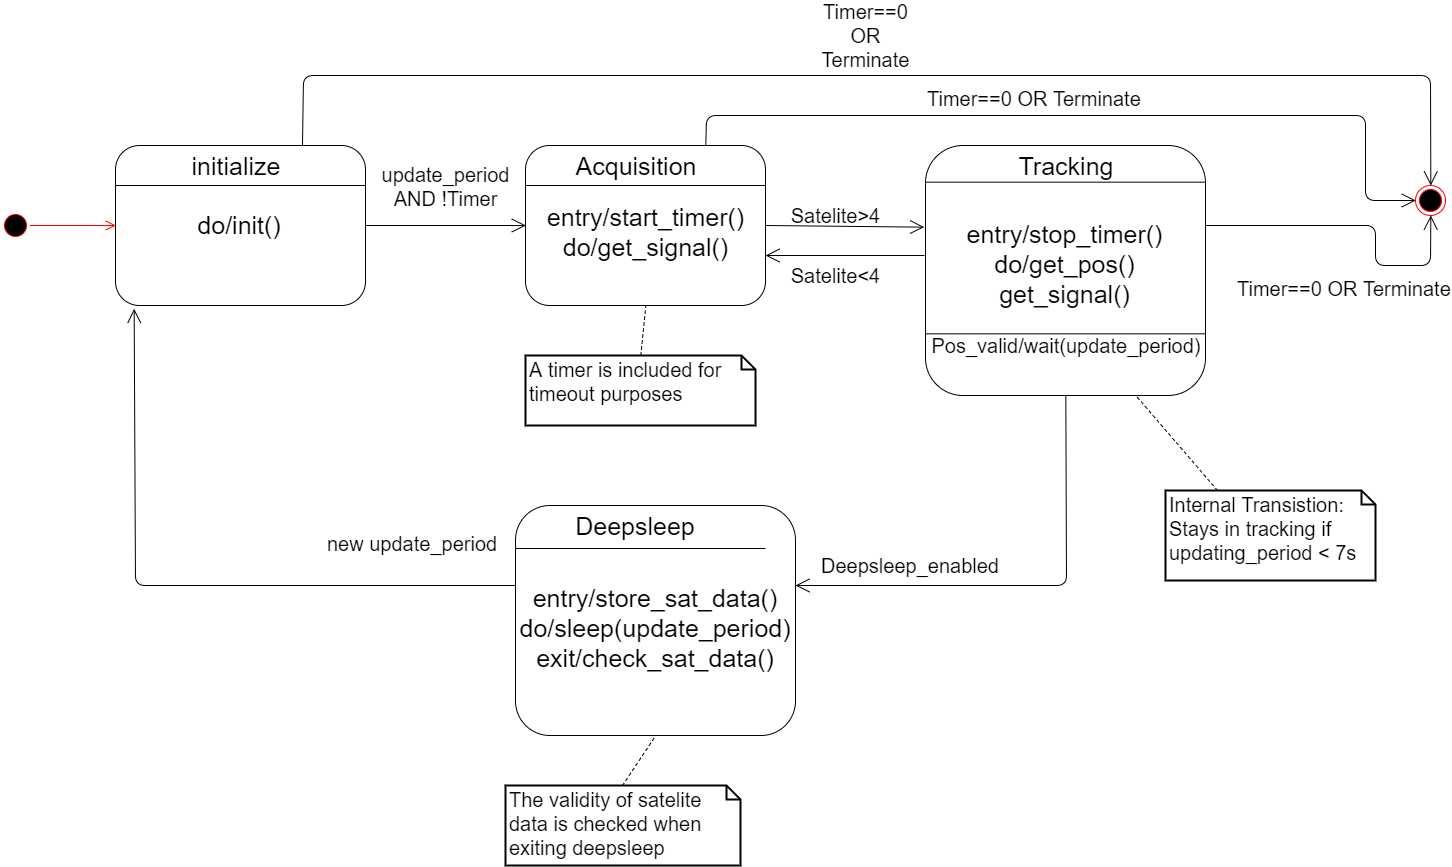
\includegraphics[height=4.5cm]{Project_Report/Images/Energymodel.png}
\caption{State diagram of the LoPy during a positional fix request}
\label{fig:LoPystate}
\end{figure}


 
 
The average current consumption is then calculated for each waveform by using Ohm's law.The python script uses a simple energy model to calculate the energy consumption over a fix period. A fix period is defined as the duration the microcontroller use to acquire a fix:
\begin{equation}
E_{fixperiod} = P_{fixperiod}*T_{fixperiod}
\end{equation}
During a fix period, the microcontroller transitions between the states in \ref{fig:LoPystate}. The total energy consumption $E_{fixperiod}$ can then be written as the sum of the energy of each state:

\begin{equation}
E_{fixperiod} = P_{Idle}*T_{Idle} + P_{Acquisition}*T_{Acquisition} + P_{Tracking}*T_{Tracking} + P_{Deepsleep}*T_{Deepsleep}
\end{equation}

The total energy consumption over a duration t is given by the energy consumption of a fix period multiplied by the number of periods during the duration t.

\begin{equation}
 E_{total} = E_{fixperiod}* \frac{t}{fixperiod}
\end{equation}

The python scripts generates an Excel sheet with the data:

\begin{figure}[H]
\centering
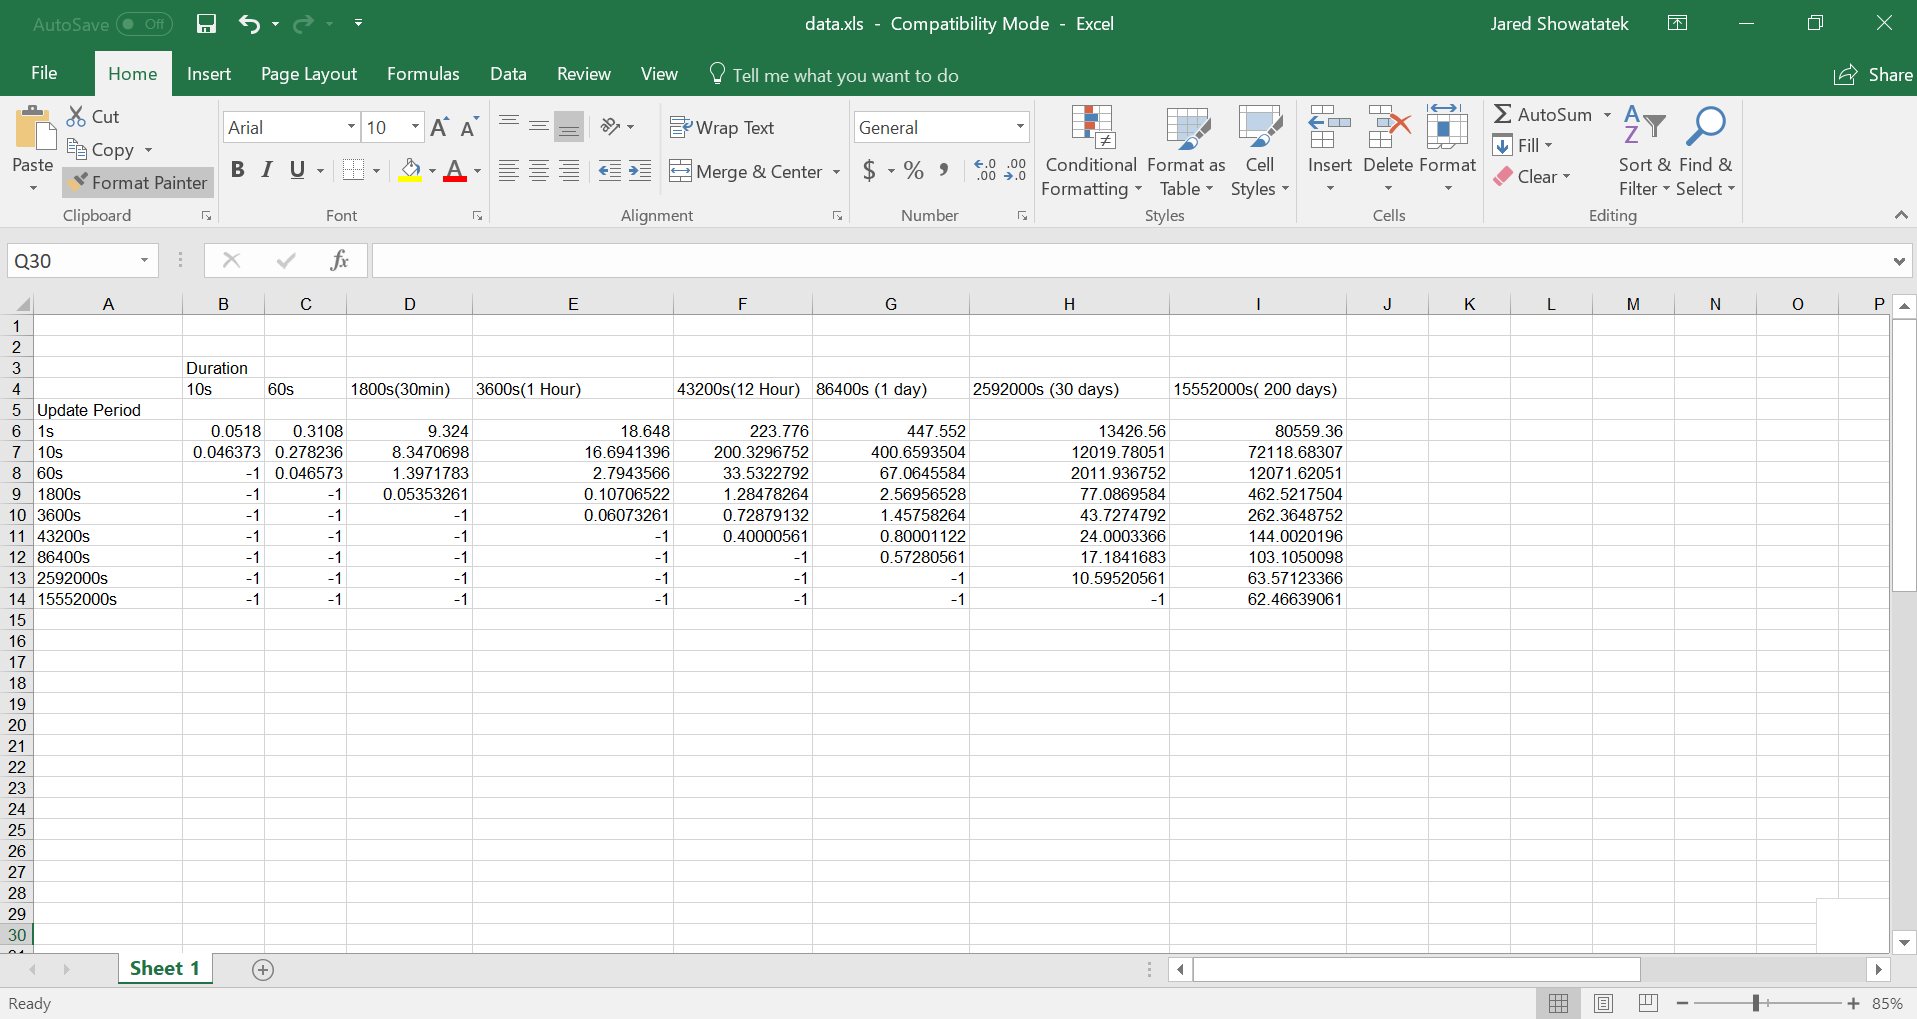
\includegraphics[height=4.5cm]{Project_Report/Images/Excel_sample.PNG}
\caption{Figure showing the generated Excel sheet}
\label{fig:Excelsample}
\end{figure}


